\documentclass[12pt, twoside,a4paper]{article}
\oddsidemargin = 10pt
\textwidth = 430pt

\usepackage{fullpage}	 %to make smaller margins
\usepackage{graphicx}
%\usepackage[utf8]{inputenc}
%\usepackage[T1]{fontenc}
%\usepackage{url}

\usepackage[hidelinks]{hyperref}
\usepackage{pdfpages}
\usepackage{placeins}
\usepackage{graphicx}
\usepackage[font=small,labelfont=bf]{caption}
\usepackage{subfig}

%\usepackage{subcaption}
\usepackage{enumerate}
\usepackage{amsmath}
\usepackage{listings} %for showing program code
\usepackage{bm}
\usepackage{wrapfig}
\usepackage{lipsum}
\usepackage{float}
\usepackage{titlesec}	
\usepackage{amsfonts}
\usepackage{amssymb}
\usepackage[comma,authoryear]{natbib}
\usepackage{epstopdf}
\usepackage{array}
\usepackage{blindtext}

%\titlespacing*{\chapter}{0pt}{-10pt}{20pt}
%\titleformat{\chapter}[display]{\normalfont\huge\bfseries}{}{35pt}{}

\setlength{\intextsep}{0pt} %to make wrapfigures beautiful
%\setlength{\oddsidemargin}{0.5cm}
%\setlength{\evensidemargin}{-0.5cm}
\begin{document}
This two weeks progress. 

\textbf{Documents}: Finished Related Work and started Implementation sections.

\textbf{Code}: I investigated more on the possible sampling patterns that are used in the models, as well as reasoning on the formula for efficiently integrating the equations.

At the end I came up with this formula:
$$
L(\mathbf{x}_o, \vec{\omega}_o) = \frac{A_{circle}}{k}\sum_{i = 1}^{k}S_i(\mathbf{x}_i,\mathbf{x}_o,\vec{\mathbf{\omega}}_i, \vec{\mathbf{\omega}}_o) \; (n_i\cdot \vec{\mathbf{\omega}}_i) \; F_t(n_i,\vec{\mathbf{\omega}}_i)
$$

where $A_{circle}$ is the area of the circle in world space. I used the following two sampling patterns, an uniform one and an exponential one. Both are generated using Hammersmith points, the second is modified by converting the points to polar coordinates and then applying the following formula to the radius:

$$
r^{*} =  \frac{e^{\sigma r} - 1}{e^{\sigma} - 1}; 
$$

We used $\sigma = 2$ for all tests. We tested different radiuses in texture space with both the exponential and uniform pattern.

\clearpage
\begin{figure}[!ht]
\centering
\subfloat[Uniform]{
  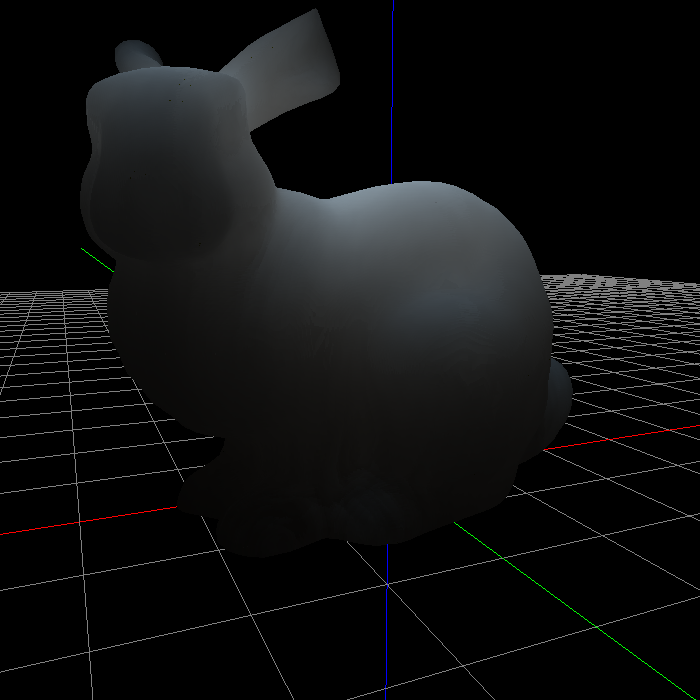
\includegraphics[width=0.33 \linewidth]{radius_03_500_uniform.png}
  \label{fig:ss2}
} 
\subfloat[Exponential]{
  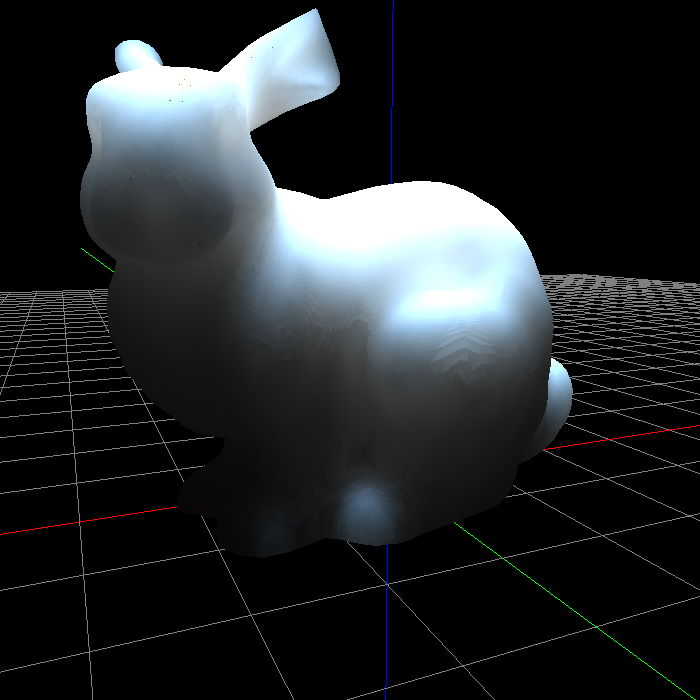
\includegraphics[width=0.33 \linewidth]{radius_03_500.png}
  \label{fig:ss3}
}
\subfloat[Reference]{
  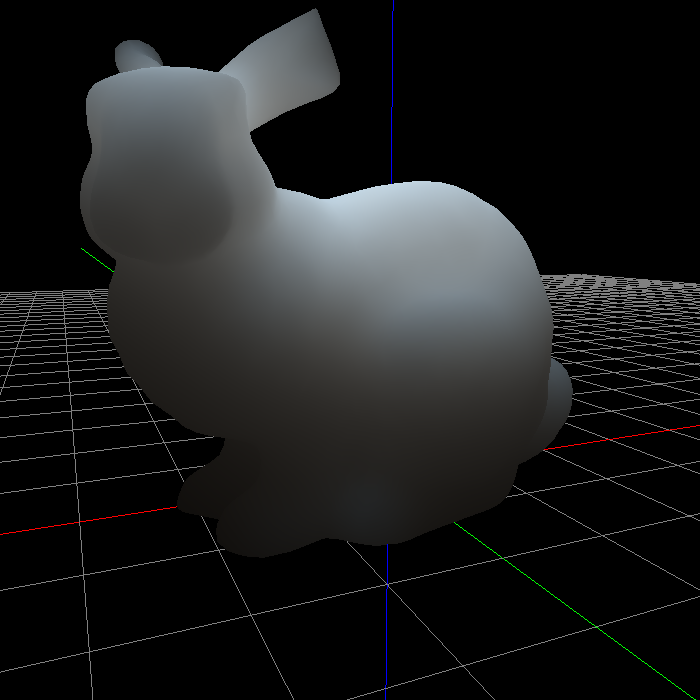
\includegraphics[width=0.33 \linewidth]{reference}
  \label{fig:ss3}
} 
 
\caption{Difference between sampling patterns vs. reference. Jensen dipole, $r = 0.3$, 300 samples.}
\label{fig:img}
\end{figure}

\begin{figure}[!ht]
\centering
\subfloat[Uniform]{
  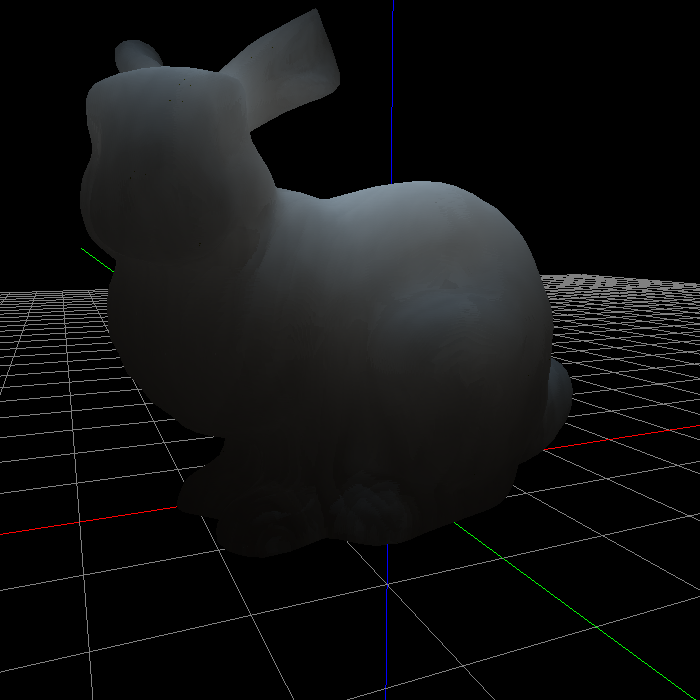
\includegraphics[width=0.33 \linewidth]{radius_05_500_uniform.png}
  \label{fig:ss2}
} 
\subfloat[Exponential]{
  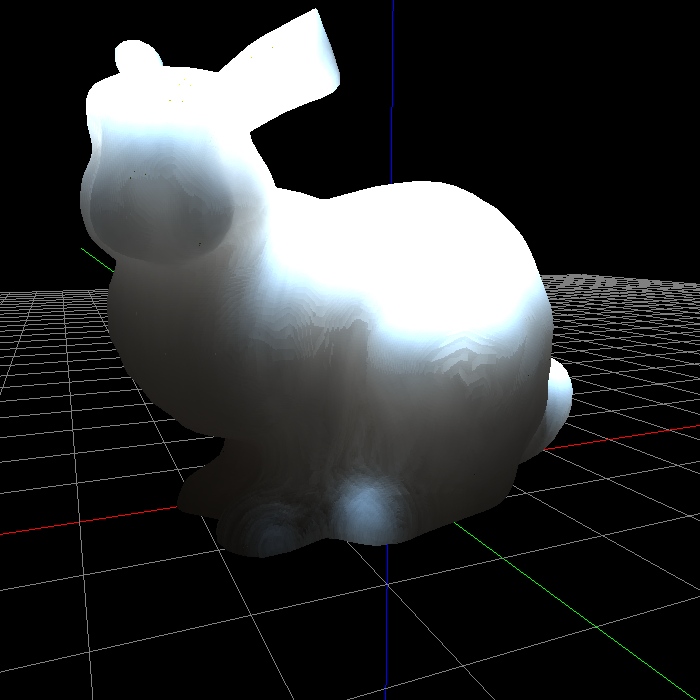
\includegraphics[width=0.33 \linewidth]{radius_05_500.png}
  \label{fig:ss3}
}
\subfloat[Reference]{
  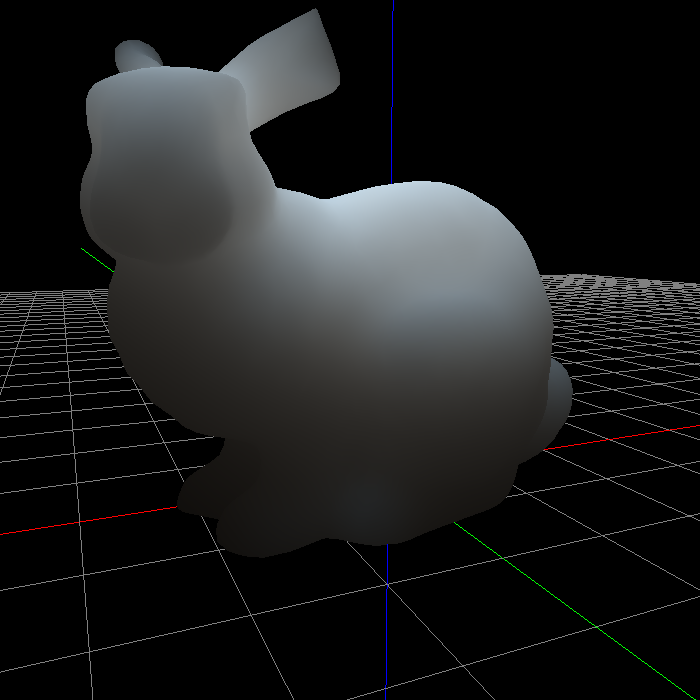
\includegraphics[width=0.33 \linewidth]{reference}
  \label{fig:ss3}
} 
 
\caption{Difference between sampling patterns vs. reference. Jensen dipole, $r = 0.5$, 300 samples.}
\label{fig:img}
\end{figure}
\clearpage

In the implementation with directional dipole, there are still some artifacts, that need investigation.
\begin{figure}[!ht]
\centering
\subfloat[Uniform]{
  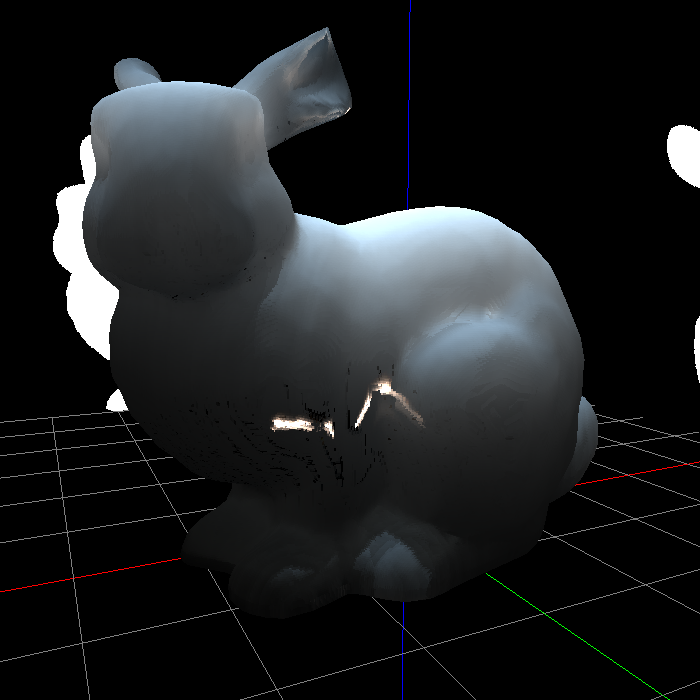
\includegraphics[width=0.5 \linewidth]{bunny_jeppe_uniform.png}
  \label{fig:ss2}
} 
\subfloat[Exponential]{
  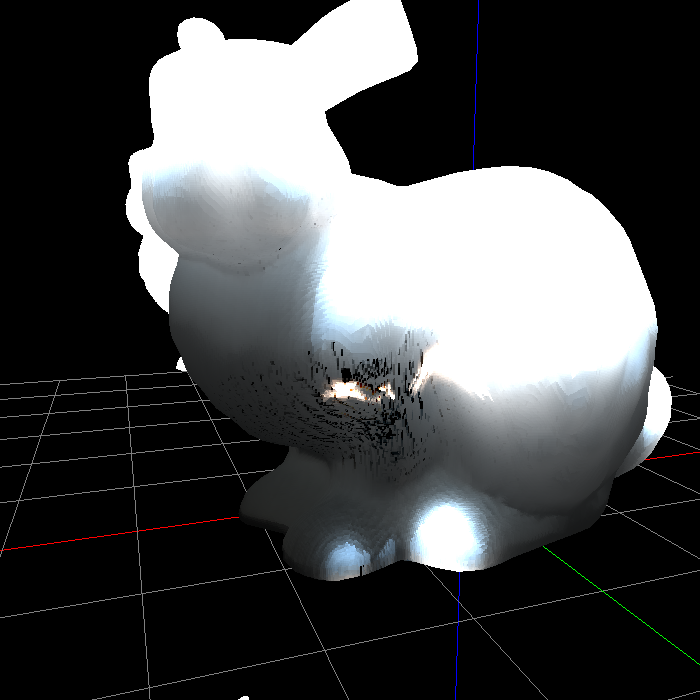
\includegraphics[width=0.5 \linewidth]{bunny_jeppe_exp.png}
  \label{fig:ss3}
}
 
\caption{Difference between sampling patterns. Directional dipole, $r = 0.5$, 1000 samples.}
\label{fig:img}
\end{figure}


%\section{Future work}
%My schedule for next week:
%\begin{itemize}
	%\item Solve banding artifacts that are still present (seem to be caused by sampling too close to the point of interest)
	%\item Try to add the directional dipole (at the moment I am testing Jensen)
	%\item Find reasonable formulas for the epsilons (at the moment they must be set manually)
	%\item Focus a little bit more on the report (deliver previous work section and reorganizing some notes on the implementation)
%\end{itemize}

\end{document}
